\newpage
\section{Monetary Transition Channels} \label{MonetaryTransitionChannels}
In his paper \footcite[See.][]{Mishkin1996}, Mishkin gives an overview of the transmission mechanisms of monetary policy in economy. Most importatn channels are namely interest rate channel, asset prices and credit channel. In the following sections we review this paper and explain every channel in detail. 

\subsection{Interest Rate}
Interest rate channel is explained with the traditional Keynesian \ac{ISLM} and shows the effects of a monetary expansion as follows:
  \[M \uparrow \implies r \downarrow \implies I \uparrow \implies Y \uparrow\]
where $ M \uparrow $ indicates expansionary monetary policy which leads to fall in real interest rate $r$, which lowers the cost of capital, causing rise in investment spending $I$, therefore resulting in increase in output $y$.
This is equal to a shift to the right of IS curve in IS-LM graph. One should notice that the real interest rate is a function of the nominal interest rate and inflation such that an increase in inflation causes a decrease in real interest rate. As an example even if the nominal interest rate is at a floor zero an increase in money supply can cause an increase in expected price which respectively decreases the real interest rate.

\subsection{Asset Price Channels}
Exchange Rate:
According to Mishkin \footcite[See.][]{Mishkin1996} the exchange rate channel can be illustrated as follows:
 \[M \uparrow \implies r \downarrow \implies E \downarrow \implies NX \uparrow\ Y \uparrow\]
An expansionary monetary policy least to fall in domestic real interest rate. As a consequence domestic currency$E$  becomes less attractive in comparison to other currencies. Depreciated currency makes domestic good more attractive for export. As a result net export $NX$ raises followed by aggregate output. s
Equity Price Channels:
 Two sub-channels are introduced for equity price namely Tobin's q and Wealth Effects \footcite[See.][]{Mishkin1996}. 
Tobin's q can be summarized as following \footcite[See.][]{Mishkin1996}: 
 \[M \uparrow \implies P_e \uparrow \implies q \uparrow \implies I \uparrow \implies Y \uparrow\]
Higher equity prices $P_e$ leads to a higher $q$ factor (market value of the firm divided by replacement cost of capital). When $q$ is high companies issue equities and buy new investment goods which are relatively cheaper so investment increases. 
The wealth channel is described as follows \footcite[See.][]{Mishkin1996}: 
\[M \uparrow \implies P_e \uparrow \implies wealth \uparrow \implies consumption \uparrow \implies Y \uparrow\]
Housing and land price which is our topic of interest in this work can be categorized in this channel as equity.

\subsection{Credit Channels}
Two basic channels of monetary transmission emerged because of asymmetric information are Bank Lending and Balance Sheet channels. 
Bank Lending Channel \footcite[See.][]{Mishkin1996}:
This transmission channel is very straightforward:
 \[M \uparrow \implies bank deposits \uparrow \implies bank loans \uparrow \implies I \uparrow\ Y \uparrow\]
Increased bank reserves and available loans causes investment to rise.
Balance Sheet Channel \footcite[See.][]{Mishkin1996}:
 \[M \uparrow \implies P_e \uparrow \implies adverse selection and moral hazard \downarrow \implies lending \uparrow \implies I \uparrow \implies Y \uparrow\]
Expansionary monetary policy raises the cashflow and consequently reduces adverse selection and moral hazard (risk) and therefore more lending.

\subsection{Housing Related Transmission Channels}

Among all the channels explained in previous sections, a very concise representation of the housing market related channels are shown in Figure \ref{fig:HousingTransmission}
\begin{figure}[H]
\caption{Monetary Transmission Channels Affecting the Housing Market }\label{fig:HousingTransmission}
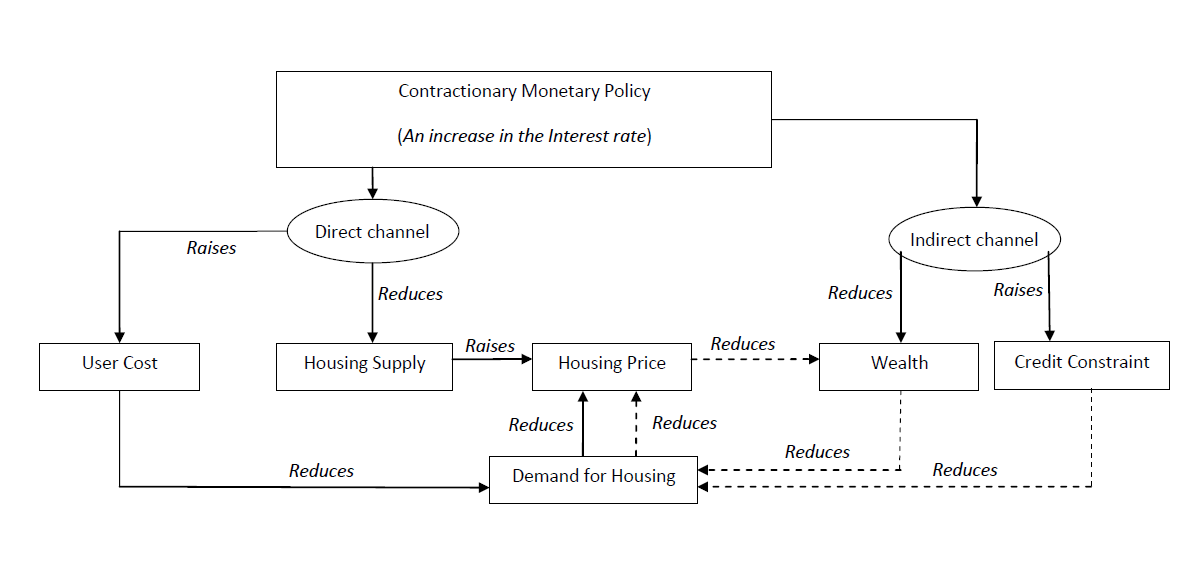
\includegraphics[width=0.9\textwidth]{HousingTransmission}
\\
\cite[Source: See][]{Wadud2009}
\end{figure}

Following his older paper on monetary transmission channels, Mishkin concentrates merely on housing market in his more recent paper~\footcite[See.][]{Mishkin1996} and explains these channels as follows:
\subsubsection{Direct Channels}
Direct Interest Rate Effects through the User Cost of Capital

The user cost of housing capital can be described as ~\footcite[See.][]{Mishkin2007}
 \[ uc = hp((1-t)i - \pi_e) - (/pi_h - /pi_e) + \delta \]
 whre $uc$ is user cost of capital, $hp$ is the relative purchase price of new housing capital, $i$ is the mortgage rate and $/pi_h$ and $/pi_e$ are the appreciation of housing prices and real inflation. $\delta$ is depreciation rate for housing. The formula also deductible mortgage interest by adjusting the nominal mortgage rate by the marginal tax rate $t$. after tax real interest rate. One can see that when the interest rate raises the user cost of capital raises  and consequently the demand for housing decreases. The fall in demand result in a fall in supply and consequently aggregate demand. Looking more precisely in $(/pi_h - /pi_e)$ part of user cost equation one can see the effect of interest rate. When interest rate raises the expected appreciation of housing price falls and therefore the current user cost of capital increases which in turn result in decline in demand. 

Interest Rate Effect on Supply \footcite[See.][]{Mishkin2007}
Higher short-term rates, which increase cost of supply and decreases housing activity.

\subsubsection{Indirect Channels}
Wealth Effects \footcite[See.][]{Mishkin2007}
There evidences proving an increase in wealth should have positive effect on consumption\footcite[See.][]{Mishkin2007}. As we know from previous section an expansionary monetary policy can increase the demand for housing which normally leads to in increase in house price. Therefore, this results to an increase in total wealth and consequently aggregate demand.
Balance Sheet, Credit-Channel Effects on Consumer Spending \footcite[See.][]{Mishkin2007}
An increase in house price improves the house hold balance sheet and reduces the risk for the credit giver as explained in previous sections.
In Figure on can see a general plot of changes in the variables introduecd in .
\begin{figure}[H]
\caption{Interest Rate, Government Spending and House Price in Germany in Years 2000-2020}
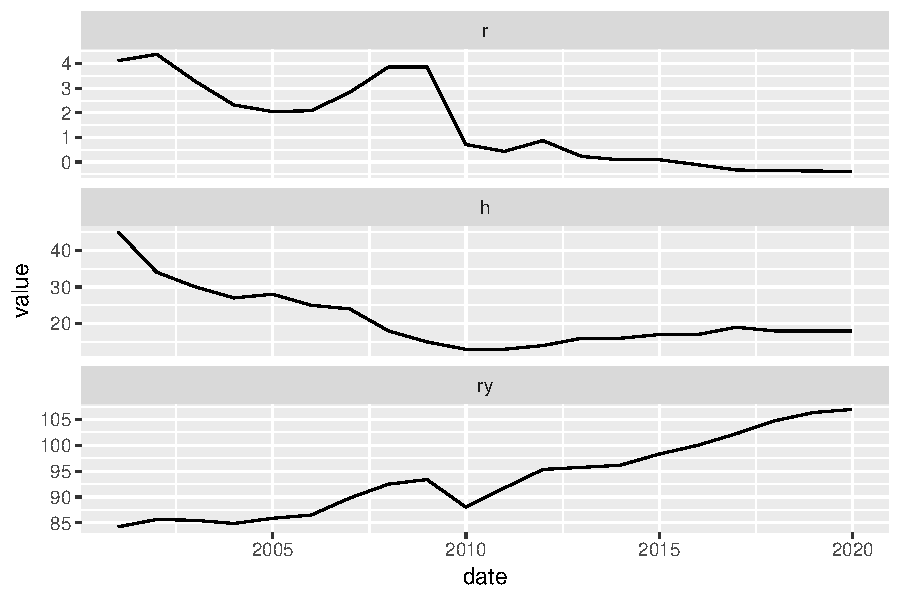
\includegraphics[width=0.9\textwidth]{interestRateOnOutput}
\\
\cite[Quelle: Own Graph][]{FOM}
\end{figure}

As one can see a has lead to house price to decrease.

